%% bare_jrnl_compsoc.tex
%% V1.4b
%% 2015/08/26
%% by Michael Shell
%% See:
%% http://www.michaelshell.org/
%% for current contact information.
%%
%% This is a skeleton file demonstrating the use of IEEEtran.cls
%% (requires IEEEtran.cls version 1.8b or later) with an IEEE
%% Computer Society journal paper.
%%
%% Support sites:
%% http://www.michaelshell.org/tex/ieeetran/
%% http://www.ctan.org/pkg/ieeetran
%% and
%% http://www.ieee.org/

%%*************************************************************************
%% Legal Notice:
%% This code is offered as-is without any warranty either expressed or
%% implied; without even the implied warranty of MERCHANTABILITY or
%% FITNESS FOR A PARTICULAR PURPOSE! 
%% User assumes all risk.
%% In no event shall the IEEE or any contributor to this code be liable for
%% any damages or losses, including, but not limited to, incidental,
%% consequential, or any other damages, resulting from the use or misuse
%% of any information contained here.
%%
%% All comments are the opinions of their respective authors and are not
%% necessarily endorsed by the IEEE.
%%
%% This work is distributed under the LaTeX Project Public License (LPPL)
%% ( http://www.latex-project.org/ ) version 1.3, and may be freely used,
%% distributed and modified. A copy of the LPPL, version 1.3, is included
%% in the base LaTeX documentation of all distributions of LaTeX released
%% 2003/12/01 or later.
%% Retain all contribution notices and credits.
%% ** Modified files should be clearly indicated as such, including  **
%% ** renaming them and changing author support contact information. **
%%*************************************************************************


% *** Authors should verify (and, if needed, correct) their LaTeX system  ***
% *** with the testflow diagnostic prior to trusting their LaTeX platform ***
% *** with production work. The IEEE's font choices and paper sizes can   ***
% *** trigger bugs that do not appear when using other class files.       ***                          ***
% The testflow support page is at:
% http://www.michaelshell.org/tex/testflow/


\documentclass[10pt,journal,compsoc]{IEEEtran}
\usepackage{graphicx}
%
% If IEEEtran.cls has not been installed into the LaTeX system files,
% manually specify the path to it like:
% \documentclass[10pt,journal,compsoc]{../sty/IEEEtran}





% Some very useful LaTeX packages include:
% (uncomment the ones you want to load)


% *** MISC UTILITY PACKAGES ***
%
%\usepackage{ifpdf}
% Heiko Oberdiek's ifpdf.sty is very useful if you need conditional
% compilation based on whether the output is pdf or dvi.
% usage:
% \ifpdf
%   % pdf code
% \else
%   % dvi code
% \fi
% The latest version of ifpdf.sty can be obtained from:
% http://www.ctan.org/pkg/ifpdf
% Also, note that IEEEtran.cls V1.7 and later provides a builtin
% \ifCLASSINFOpdf conditional that works the same way.
% When switching from latex to pdflatex and vice-versa, the compiler may
% have to be run twice to clear warning/error messages.






% *** CITATION PACKAGES ***
%
\ifCLASSOPTIONcompsoc
  % IEEE Computer Society needs nocompress option
  % requires cite.sty v4.0 or later (November 2003)
  \usepackage[nocompress]{cite}
\else
  % normal IEEE
  \usepackage{cite}
\fi
% cite.sty was written by Donald Arseneau
% V1.6 and later of IEEEtran pre-defines the format of the cite.sty package
% \cite{} output to follow that of the IEEE. Loading the cite package will
% result in citation numbers being automatically sorted and properly
% "compressed/ranged". e.g., [1], [9], [2], [7], [5], [6] without using
% cite.sty will become [1], [2], [5]--[7], [9] using cite.sty. cite.sty's
% \cite will automatically add leading space, if needed. Use cite.sty's
% noadjust option (cite.sty V3.8 and later) if you want to turn this off
% such as if a citation ever needs to be enclosed in parenthesis.
% cite.sty is already installed on most LaTeX systems. Be sure and use
% version 5.0 (2009-03-20) and later if using hyperref.sty.
% The latest version can be obtained at:
% http://www.ctan.org/pkg/cite
% The documentation is contained in the cite.sty file itself.
%
% Note that some packages require special options to format as the Computer
% Society requires. In particular, Computer Society  papers do not use
% compressed citation ranges as is done in typical IEEE papers
% (e.g., [1]-[4]). Instead, they list every citation separately in order
% (e.g., [1], [2], [3], [4]). To get the latter we need to load the cite
% package with the nocompress option which is supported by cite.sty v4.0
% and later. Note also the use of a CLASSOPTION conditional provided by
% IEEEtran.cls V1.7 and later.





% *** GRAPHICS RELATED PACKAGES ***
%
\ifCLASSINFOpdf
  % \usepackage[pdftex]{graphicx}
  % declare the path(s) where your graphic files are
  % \graphicspath{{../pdf/}{../jpeg/}}
  % and their extensions so you won't have to specify these with
  % every instance of \includegraphics
  % \DeclareGraphicsExtensions{.pdf,.jpeg,.png}
\else
  % or other class option (dvipsone, dvipdf, if not using dvips). graphicx
  % will default to the driver specified in the system graphics.cfg if no
  % driver is specified.
  % \usepackage[dvips]{graphicx}
  % declare the path(s) where your graphic files are
  % \graphicspath{{../eps/}}
  % and their extensions so you won't have to specify these with
  % every instance of \includegraphics
  % \DeclareGraphicsExtensions{.eps}
\fi
% graphicx was written by David Carlisle and Sebastian Rahtz. It is
% required if you want graphics, photos, etc. graphicx.sty is already
% installed on most LaTeX systems. The latest version and documentation
% can be obtained at: 
% http://www.ctan.org/pkg/graphicx
% Another good source of documentation is "Using Imported Graphics in
% LaTeX2e" by Keith Reckdahl which can be found at:
% http://www.ctan.org/pkg/epslatex
%
% latex, and pdflatex in dvi mode, support graphics in encapsulated
% postscript (.eps) format. pdflatex in pdf mode supports graphics
% in .pdf, .jpeg, .png and .mps (metapost) formats. Users should ensure
% that all non-photo figures use a vector format (.eps, .pdf, .mps) and
% not a bitmapped formats (.jpeg, .png). The IEEE frowns on bitmapped formats
% which can result in "jaggedy"/blurry rendering of lines and letters as
% well as large increases in file sizes.
%
% You can find documentation about the pdfTeX application at:
% http://www.tug.org/applications/pdftex






% *** MATH PACKAGES ***
%
%\usepackage{amsmath}
% A popular package from the American Mathematical Society that provides
% many useful and powerful commands for dealing with mathematics.
%
% Note that the amsmath package sets \interdisplaylinepenalty to 10000
% thus preventing page breaks from occurring within multiline equations. Use:
%\interdisplaylinepenalty=2500
% after loading amsmath to restore such page breaks as IEEEtran.cls normally
% does. amsmath.sty is already installed on most LaTeX systems. The latest
% version and documentation can be obtained at:
% http://www.ctan.org/pkg/amsmath





% *** SPECIALIZED LIST PACKAGES ***
%
%\usepackage{algorithmic}
% algorithmic.sty was written by Peter Williams and Rogerio Brito.
% This package provides an algorithmic environment fo describing algorithms.
% You can use the algorithmic environment in-text or within a figure
% environment to provide for a floating algorithm. Do NOT use the algorithm
% floating environment provided by algorithm.sty (by the same authors) or
% algorithm2e.sty (by Christophe Fiorio) as the IEEE does not use dedicated
% algorithm float types and packages that provide these will not provide
% correct IEEE style captions. The latest version and documentation of
% algorithmic.sty can be obtained at:
% http://www.ctan.org/pkg/algorithms
% Also of interest may be the (relatively newer and more customizable)
% algorithmicx.sty package by Szasz Janos:
% http://www.ctan.org/pkg/algorithmicx




% *** ALIGNMENT PACKAGES ***
%
%\usepackage{array}
% Frank Mittelbach's and David Carlisle's array.sty patches and improves
% the standard LaTeX2e array and tabular environments to provide better
% appearance and additional user controls. As the default LaTeX2e table
% generation code is lacking to the point of almost being broken with
% respect to the quality of the end results, all users are strongly
% advised to use an enhanced (at the very least that provided by array.sty)
% set of table tools. array.sty is already installed on most systems. The
% latest version and documentation can be obtained at:
% http://www.ctan.org/pkg/array


% IEEEtran contains the IEEEeqnarray family of commands that can be used to
% generate multiline equations as well as matrices, tables, etc., of high
% quality.




% *** SUBFIGURE PACKAGES ***
%\ifCLASSOPTIONcompsoc
%  \usepackage[caption=false,font=footnotesize,labelfont=sf,textfont=sf]{subfig}
%\else
%  \usepackage[caption=false,font=footnotesize]{subfig}
%\fi
% subfig.sty, written by Steven Douglas Cochran, is the modern replacement
% for subfigure.sty, the latter of which is no longer maintained and is
% incompatible with some LaTeX packages including fixltx2e. However,
% subfig.sty requires and automatically loads Axel Sommerfeldt's caption.sty
% which will override IEEEtran.cls' handling of captions and this will result
% in non-IEEE style figure/table captions. To prevent this problem, be sure
% and invoke subfig.sty's "caption=false" package option (available since
% subfig.sty version 1.3, 2005/06/28) as this is will preserve IEEEtran.cls
% handling of captions.
% Note that the Computer Society format requires a sans serif font rather
% than the serif font used in traditional IEEE formatting and thus the need
% to invoke different subfig.sty package options depending on whether
% compsoc mode has been enabled.
%
% The latest version and documentation of subfig.sty can be obtained at:
% http://www.ctan.org/pkg/subfig




% *** FLOAT PACKAGES ***
%
%\usepackage{fixltx2e}
% fixltx2e, the successor to the earlier fix2col.sty, was written by
% Frank Mittelbach and David Carlisle. This package corrects a few problems
% in the LaTeX2e kernel, the most notable of which is that in current
% LaTeX2e releases, the ordering of single and double column floats is not
% guaranteed to be preserved. Thus, an unpatched LaTeX2e can allow a
% single column figure to be placed prior to an earlier double column
% figure.
% Be aware that LaTeX2e kernels dated 2015 and later have fixltx2e.sty's
% corrections already built into the system in which case a warning will
% be issued if an attempt is made to load fixltx2e.sty as it is no longer
% needed.
% The latest version and documentation can be found at:
% http://www.ctan.org/pkg/fixltx2e


%\usepackage{stfloats}
% stfloats.sty was written by Sigitas Tolusis. This package gives LaTeX2e
% the ability to do double column floats at the bottom of the page as well
% as the top. (e.g., "\begin{figure*}[!b]" is not normally possible in
% LaTeX2e). It also provides a command:
%\fnbelowfloat
% to enable the placement of footnotes below bottom floats (the standard
% LaTeX2e kernel puts them above bottom floats). This is an invasive package
% which rewrites many portions of the LaTeX2e float routines. It may not work
% with other packages that modify the LaTeX2e float routines. The latest
% version and documentation can be obtained at:
% http://www.ctan.org/pkg/stfloats
% Do not use the stfloats baselinefloat ability as the IEEE does not allow
% \baselineskip to stretch. Authors submitting work to the IEEE should note
% that the IEEE rarely uses double column equations and that authors should try
% to avoid such use. Do not be tempted to use the cuted.sty or midfloat.sty
% packages (also by Sigitas Tolusis) as the IEEE does not format its papers in
% such ways.
% Do not attempt to use stfloats with fixltx2e as they are incompatible.
% Instead, use Morten Hogholm'a dblfloatfix which combines the features
% of both fixltx2e and stfloats:
%
% \usepackage{dblfloatfix}
% The latest version can be found at:
% http://www.ctan.org/pkg/dblfloatfix




%\ifCLASSOPTIONcaptionsoff
%  \usepackage[nomarkers]{endfloat}
% \let\MYoriglatexcaption\caption
% \renewcommand{\caption}[2][\relax]{\MYoriglatexcaption[#2]{#2}}
%\fi
% endfloat.sty was written by James Darrell McCauley, Jeff Goldberg and 
% Axel Sommerfeldt. This package may be useful when used in conjunction with 
% IEEEtran.cls'  captionsoff option. Some IEEE journals/societies require that
% submissions have lists of figures/tables at the end of the paper and that
% figures/tables without any captions are placed on a page by themselves at
% the end of the document. If needed, the draftcls IEEEtran class option or
% \CLASSINPUTbaselinestretch interface can be used to increase the line
% spacing as well. Be sure and use the nomarkers option of endfloat to
% prevent endfloat from "marking" where the figures would have been placed
% in the text. The two hack lines of code above are a slight modification of
% that suggested by in the endfloat docs (section 8.4.1) to ensure that
% the full captions always appear in the list of figures/tables - even if
% the user used the short optional argument of \caption[]{}.
% IEEE papers do not typically make use of \caption[]'s optional argument,
% so this should not be an issue. A similar trick can be used to disable
% captions of packages such as subfig.sty that lack options to turn off
% the subcaptions:
% For subfig.sty:
% \let\MYorigsubfloat\subfloat
% \renewcommand{\subfloat}[2][\relax]{\MYorigsubfloat[]{#2}}
% However, the above trick will not work if both optional arguments of
% the \subfloat command are used. Furthermore, there needs to be a
% description of each subfigure *somewhere* and endfloat does not add
% subfigure captions to its list of figures. Thus, the best approach is to
% avoid the use of subfigure captions (many IEEE journals avoid them anyway)
% and instead reference/explain all the subfigures within the main caption.
% The latest version of endfloat.sty and its documentation can obtained at:
% http://www.ctan.org/pkg/endfloat
%
% The IEEEtran \ifCLASSOPTIONcaptionsoff conditional can also be used
% later in the document, say, to conditionally put the References on a 
% page by themselves.




% *** PDF, URL AND HYPERLINK PACKAGES ***
%
%\usepackage{url}
% url.sty was written by Donald Arseneau. It provides better support for
% handling and breaking URLs. url.sty is already installed on most LaTeX
% systems. The latest version and documentation can be obtained at:
% http://www.ctan.org/pkg/url
% Basically, \url{my_url_here}.





% *** Do not adjust lengths that control margins, column widths, etc. ***
% *** Do not use packages that alter fonts (such as pslatex).         ***
% There should be no need to do such things with IEEEtran.cls V1.6 and later.
% (Unless specifically asked to do so by the journal or conference you plan
% to submit to, of course. )


% correct bad hyphenation here
\hyphenation{op-tical net-works semi-conduc-tor}


\begin{document}
%
% paper title
% Titles are generally capitalized except for words such as a, an, and, as,
% at, but, by, for, in, nor, of, on, or, the, to and up, which are usually
% not capitalized unless they are the first or last word of the title.
% Linebreaks \\ can be used within to get better formatting as desired.
% Do not put math or special symbols in the title.
\title{Mental Health Prediction using \\ Quantum-enhanced Machine Learning}
%
%
% author names and IEEE memberships
% note positions of commas and nonbreaking spaces ( ~ ) LaTeX will not break
% a structure at a ~ so this keeps an author's name from being broken across
% two lines.
% use \thanks{} to gain access to the first footnote area
% a separate \thanks must be used for each paragraph as LaTeX2e's \thanks
% was not built to handle multiple paragraphs
%
%
%\IEEEcompsocitemizethanks is a special \thanks that produces the bulleted
% lists the Computer Society journals use for "first footnote" author
% affiliations. Use \IEEEcompsocthanksitem which works much like \item
% for each affiliation group. When not in compsoc mode,
% \IEEEcompsocitemizethanks becomes like \thanks and
% \IEEEcompsocthanksitem becomes a line break with idention. This
% facilitates dual compilation, although admittedly the differences in the
% desired content of \author between the different types of papers makes a
% one-size-fits-all approach a daunting prospect. For instance, compsoc 
% journal papers have the author affiliations above the "Manuscript
% received ..."  text while in non-compsoc journals this is reversed. Sigh.

\author{Neha~Shaikh, Praveen~Kumar~Thanniru, 
        Sadakhya~Narnur,\
        and~Rahul~Reddy~Parupati% <-this % stops a space
\IEEEcompsocitemizethanks{\IEEEcompsocthanksitem Neha Shaikh
 was with the Department
of Applied Data Science, San Jose State University, San Jose,
CA, 95192.\protect\\
% note need leading \protect in front of \\ to get a newline within \thanks as
% \\ is fragile and will error, could use \hfil\break instead.
E-mail: neha.shaikh@sjsu.edu
\IEEEcompsocthanksitem Praveen Kumar 
 was with the Department
of Applied Data Science, San Jose State University, San Jose,
CA, 95192.\protect\\
% note need leading \protect in front of \\ to get a newline within \thanks as
% \\ is fragile and will error, could use \hfil\break instead.
E-mail: praveenkumar.thanniru@sjsu.edu
\IEEEcompsocthanksitem Sadakhya Narnur
 are with the Department
of Applied Data Science, San Jose State University, San Jose,
CA, 95192.\protect\\
% note need leading \protect in front of \\ to get a newline within \thanks as
% \\ is fragile and will error, could use \hfil\break instead.
E-mail: sadakhya.narnur@sjsu.edu
\IEEEcompsocthanksitem Rahul Reddy Parupati 
 was with the Department
of Applied Data Science, San Jose State University, San Jose,
CA, 95192.\protect\\
% note need leading \protect in front of \\ to get a newline within \thanks as
% \\ is fragile and will error, could use \hfil\break instead.
E-mail: rahulreddy.parupati@sjsu.edu
}% <-this % stops an unwanted space
\thanks{Manuscript received November 28, 2022}}

% note the % following the last \IEEEmembership and also \thanks - 
% these prevent an unwanted space from occurring between the last author name
% and the end of the author line. i.e., if you had this:
% 
% \author{....lastname \thanks{...} \thanks{...} }
%                     ^------------^------------^----Do not want these spaces!
%
% a space would be appended to the last name and could cause every name on that
% line to be shifted left slightly. This is one of those "LaTeX things". For
% instance, "\textbf{A} \textbf{B}" will typeset as "A B" not "AB". To get
% "AB" then you have to do: "\textbf{A}\textbf{B}"
% \thanks is no different in this regard, so shield the last } of each \thanks
% that ends a line with a % and do not let a space in before the next \thanks.
% Spaces after \IEEEmembership other than the last one are OK (and needed) as
% you are supposed to have spaces between the names. For what it is worth,
% this is a minor point as most people would not even notice if the said evil
% space somehow managed to creep in.



% The paper headers
\markboth{DATA 245 Machine Learning Technologies, November~2022}%
{Shell \MakeLowercase{\textit{et al.}}: Bare Demo of IEEEtran.cls for Computer Society Journals}
% The only time the second header will appear is for the odd numbered pages
% after the title page when using the twoside option.
% 
% *** Note that you probably will NOT want to include the author's ***
% *** name in the headers of peer review papers.                   ***
% You can use \ifCLASSOPTIONpeerreview for conditional compilation here if
% you desire.



% The publisher's ID mark at the bottom of the page is less important with
% Computer Society journal papers as those publications place the marks
% outside of the main text columns and, therefore, unlike regular IEEE
% journals, the available text space is not reduced by their presence.
% If you want to put a publisher's ID mark on the page you can do it like
% this:
%\IEEEpubid{0000--0000/00\$00.00~\copyright~2015 IEEE}
% or like this to get the Computer Society new two part style.
%\IEEEpubid{\makebox[\columnwidth]{\hfill 0000--0000/00/\$00.00~\copyright~2015 IEEE}%
%\hspace{\columnsep}\makebox[\columnwidth]{Published by the IEEE Computer Society\hfill}}
% Remember, if you use this you must call \IEEEpubidadjcol in the second
% column for its text to clear the IEEEpubid mark (Computer Society jorunal
% papers don't need this extra clearance.)



% use for special paper notices
%\IEEEspecialpapernotice{(Invited Paper)}



% for Computer Society papers, we must declare the abstract and index terms
% PRIOR to the title within the \IEEEtitleabstractindextext IEEEtran
% command as these need to go into the title area created by \maketitle.
% As a general rule, do not put math, special symbols or citations
% in the abstract or keywords.
\IEEEtitleabstractindextext{%
\begin{abstract}
Mental disorders are more prevalent than heart diseases and diabetes. But there is very little importance given to this issue. With the advancements in AI, this could be an area that will benefit people to create awareness about their mental health. Combining the predictive ability of machine learning with knowledge of which factors could possibly affect mental well-being, a prediction could be made. Though a number of prior researches were made in this field, due to the dimensional constraints very few features were considered for prediction. This reduction in features can affect the accuracy of predictions which will be addressed in this project. The key is to make predictions in a higher dimensional feature space and analyze how efficient and accurate they are. Quantum enhanced Machine learning algorithms are employed to quantitatively estimate mental health based on a number of factors like age, sex, working condition, job, coworkers, etc. A mental health dataset with 27 features is used and modeled with QSVM ( Quantum Support Vector Machine). Qiskit, an open-source SDK package in python is used for working with these algorithms. An assessment of the prediction accuracy and precision is made to gauge the performance of QML models chosen for this problem.

\end{abstract}

% Note that keywords are not normally used for peerreview papers.
\begin{IEEEkeywords}
Quantum-enhanced ML, QSVM, Curse of Dimensionality, Hilbert Space
\end{IEEEkeywords}}


% make the title area
\maketitle


% To allow for easy dual compilation without having to reenter the
% abstract/keywords data, the \IEEEtitleabstractindextext text will
% not be used in maketitle, but will appear (i.e., to be "transported")
% here as \IEEEdisplaynontitleabstractindextext when the compsoc 
% or transmag modes are not selected <OR> if conference mode is selected 
% - because all conference papers position the abstract like regular
% papers do.
\IEEEdisplaynontitleabstractindextext
% \IEEEdisplaynontitleabstractindextext has no effect when using
% compsoc or transmag under a non-conference mode.



% For peer review papers, you can put extra information on the cover
% page as needed:
% \ifCLASSOPTIONpeerreview
% \begin{center} \bfseries EDICS Category: 3-BBND \end{center}
% \fi
%
% For peerreview papers, this IEEEtran command inserts a page break and
% creates the second title. It will be ignored for other modes.
\IEEEpeerreviewmaketitle



\IEEEraisesectionheading{\section{Introduction}\label{sec:introduction}}
% Computer Society journal (but not conference!) papers do something unusual
% with the very first section heading (almost always called "Introduction").
% They place it ABOVE the main text! IEEEtran.cls does not automatically do
% this for you, but you can achieve this effect with the provided
% \IEEEraisesectionheading{} command. Note the need to keep any \label that
% is to refer to the section immediately after \section in the above as
% \IEEEraisesectionheading puts \section within a raised box.




% The very first letter is a 2 line initial drop letter followed
% by the rest of the first word in caps (small caps for compsoc).
% 
% form to use if the first word consists of a single letter:
% \IEEEPARstart{A}{demo} file is ....
% 
% form to use if you need the single drop letter followed by
% normal text (unknown if ever used by the IEEE):
% \IEEEPARstart{A}{}demo file is ....
% 
% Some journals put the first two words in caps:
% \IEEEPARstart{T}{his demo} file is ....
% 
% Here we have the typical use of a "T" for an initial drop letter
% and "HIS" in caps to complete the first word.
\IEEEPARstart{T}{he} growing stress and responsibilities are often presumed to be common in our busy lives. However, to what extent it affects our Mental health is often overlooked. Many don't realize the risk of them being on the edge of mental illness. We often come across biological mental disorders that have genetic factors involved. But mental health is a broader spectrum that involves any psychological imbalance that starts to affect our thoughts, feelings, and actions. Despite one never facing adverse life experiences like trauma, abuse or violence can still be vulnerable. This makes it clear that a person’s mental health changes with time, based on many factors. Some of the factors can be early life experiences, strenuous working hours, economic burdens, social anxiety, and even physical health. This leads to a need for awareness of emotional and mental well-being. An assessment of one's sanity from time to time would help in alerting them of any need for help or treatment and thereby directing their lifestyle for overall health. 

\quad This project is based on idea where a prediction could be made of mental health as a consequence of multiple factors like age, family history, working conditions, employment, etc. Putting Machine learning into work for this project would help in predicting with greater accuracy. In ML predictions a larger number of features increase predictive modeling tasks. In order to overcome this computational overhead, dimensionality reduction referring to the reduced number of input variables is often considered. However, dimensionality reduction could be seen as a drawback that affects the predictions, often called the Curse of Dimensionality. Hence in order to extend the prediction from the euclidean vector space to higher dimensional Hilbert space to consider more features, Quantum computing  will be introduced to machine learning which is Quantum-enhanced Machine learning. This can be seen as the execution of machine learning computations on a quantum computer. It can be seen as an enhancement over machine learning prediction as it not only overcomes the dimensionality limitations but also does the computations with greater speed and improves data storage done by algorithms.

\subsection{Objective}
The objective is to prove that the QEML method will enhance and improve the ability of the traditional machine learning algorithms. The data set is selected  from the CDC website that describes different features which can be considered risk factors in mental health predictions. Aim would be to explore all the possible correlations between the features and use as many required for better prediction of whether treatment is required for a particular person's record. 

\quad To address the problem statement, we are using a super powerful quantum variants of machine learning classification algorithms: Support Vector Machine through hamming distance metrics in quantum feature space.

\section{Theoretical bases and literature review}
% needed in second column of first page if using \IEEEpubid
%\IEEEpubidadjcol

\subsection{Definition of the problem}
This study focuses on predicting the mental health of a person based on the features. In our study, we will treat the classic Machine Learning algorithms like Support Vector Machines with Quantum Computing and analyze the degree of risk a person experiences regarding his/her mental health issues.

\subsection{Theoretical background of the problem}
Pattern recognition is used in machine learning, which is a data-dependent approach for datasets of a certain size. However, as the size and quantity of features for the given case study increase, performance reduces clearly for both regression and classification machine learning algorithms.  This issue is also referred to as the Curse of Dimensionality, has severely increased runtimes and caused quadratic growth in machine learning methods. This issue stems from how data is stored in the first place. The states and characteristics of specific vectors are positioned in classical feature space for classical machine learning. The kernel operations and performance of some machine learning algorithms are inhibited by exponential storage and runtime due to this feature space. To ease the strain of exponential storage and so create a quantum feature space, it has recently been suggested to use quantum computing. The simplest answer is to convert classical states into quantum states, which can be stored more effectively. 

\subsection{Literature Review}
The current problem falls under the classification and in the presence of a number of algorithms for classification it is considered that SVM and KNN besides Random Forest are the best performing. This study tried clustering models to identify the number of possible clusters before deciding on modeling[1].This research was more focused on classifying different target groups that were vulnerable.

\quad In a similar research Predicting Mental Health Illness [2] using Machine Learning algorithms it was carried out with five algorithms namely Logistic Regression, K-NN Classifier, Decision Tree Classifier, Random Forest and Stacking. The study shows k-NN had comparably good accuracy for classification.

\quad In the research [3] a brief introduction on Quantum enhanced machine learning is given as a classic machine learning in the high dimension space. QSVM is implemented on breast cancer dataset which is a binary classification problem. It is observed that Quantum enhanced SVM performed better than classical ML SVM.A possible limitation on QSVM is discussed regarding the implementation of kernel models as it would be complex to implement using Quantum circuits for Radial basis kernel.

\quad A paper on Investigation of Quantum Support Vector Machine for classification [4] made a comparision of Quantum SVM performance over a quantum computer. They have encoded the data and run on QSVM circuit and later checked for the performance.They have observed that the QSVM has not performed well when they implemented it on NISQ era quantum simulator. They got a mere accuracy of 62\%. However later they proposed a mechanism which gave an improvement over it.

\subsection{Solution for our problem}
In this study, we as a team studied the Support Vector Machines methodology and understood the functionality of quantum-enhanced feature space. Following that, we declared the fundamental characteristics of quantum machine learning as a whole and the justification behind why it should outperform the conventional SVM algorithm. Thus the prediction of risk factors involved in the mental health of employees can be carried out effectively with the involvement of Quantum Computing.

\subsection{Why our solution is better}
With the application of a quantum feature space, which intensifies current Machine Learning algorithms as it uses the parallelization and the reduction of the storage space from exponential to linear, we may be able to solve the problem of determining the risk factor by incorporating quantum circuits into conventional Machine Learning, instead of using the traditional approach alone.

\section{Methodology}
\subsection{Collecting the input data}
The data in focus is any mental health related data that supports the classification. The Mental health dataset that is used for the project is taken from a survey conducted by Chirag Dodiya [5]. The survey was conducted where the responses of the people were recorded for classification purpose.

\subsection{Exploratory data analysis}

\begin{figure}[!t]
\centering
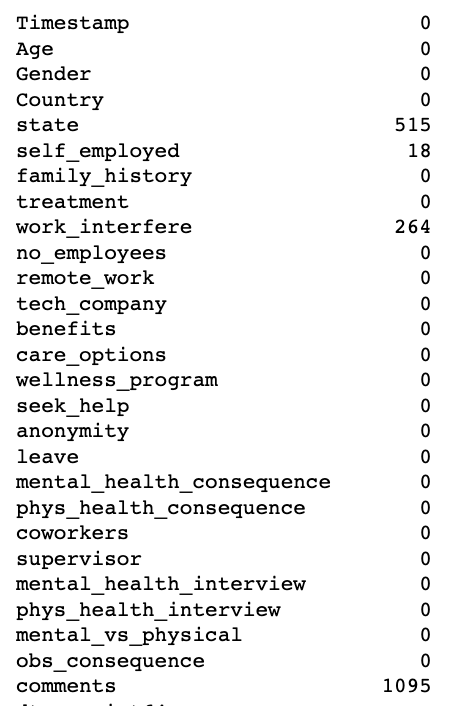
\includegraphics[width=3.5in]{5.png}
\caption{Dataframe showing the null values count for different columns}
\end{figure}

\quad Understanding the data we are going to work with helps build an efficient model. This is the second step in our project. Post understanding the project scope and defining the problem statement we have decided to use the mental health dataset for classifying a person's record. The dataset has 1260 records over 27 features namely: Timestamp, age, gender, country, state, self-employed, family history, etc.The first step of the analysis was to find the missing values in the dataset. A column summarizing the count of missing values has been observed like in Fig 1.


\quad State and comments are the two columns with the highest missing values. Further work \_interfere and self\_employed had some missing values. The gender column has a number of entries that need to be normalized and reduced to some subgroups. The age column had 4 outliers with values out of the range of the acceptable age. 

\quad A correlation matrix heatmap is used to visualize the correlations between all the features in Fig. 2. A strongest correlation is observed for treatment and work\_interference which aided us to focus more on that feature. Family\_history, benefits and care options are the next positive correlated. A distribution of age is observed with most of distribution having been teenagers. Supporting this a bar chart plotted for the age groups requiring treatment shows that people with ages 7 to 20 are showing highest need for treatment.



\begin{figure}[h]
\centering
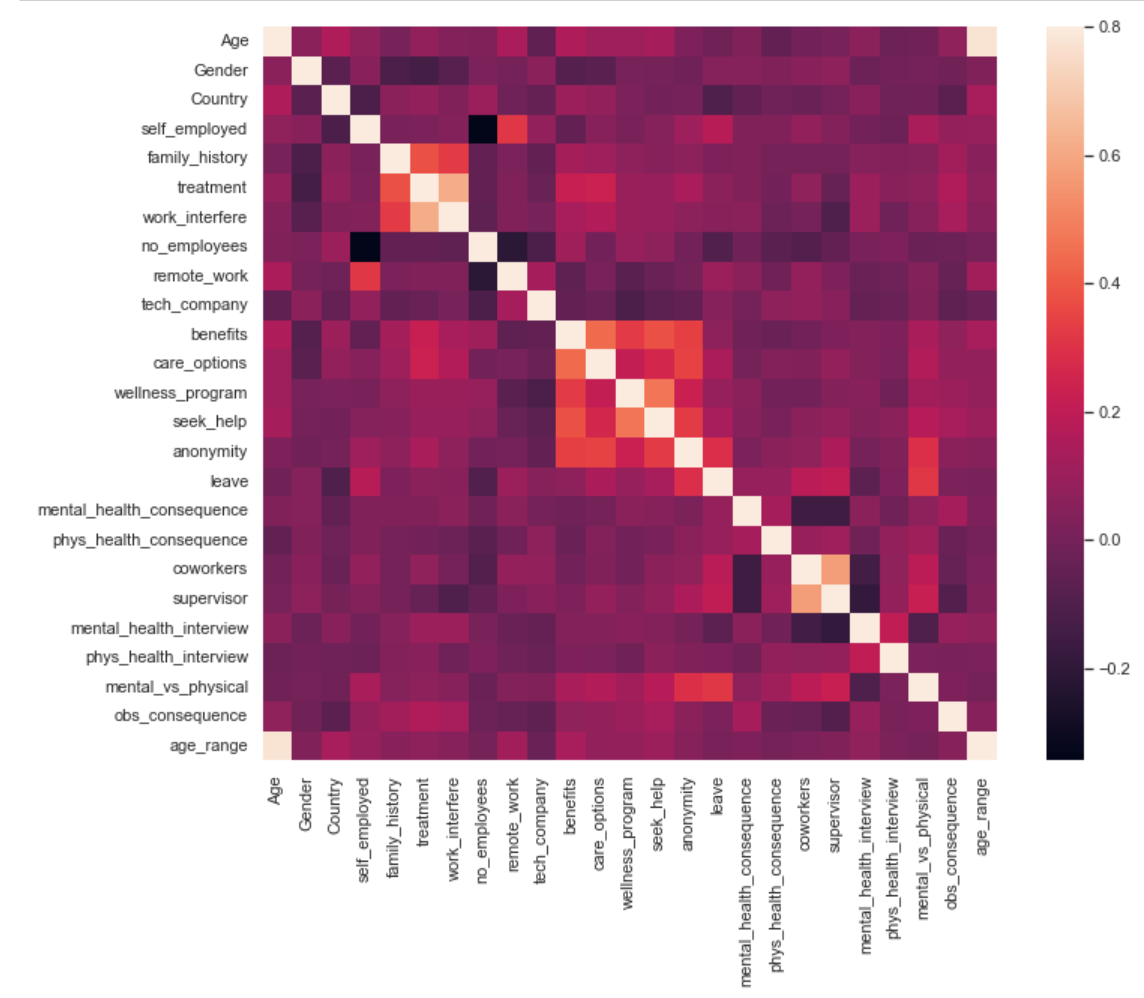
\includegraphics[width=3.5in]{heatmap.png}
\caption{Heat Map showing feature correlations}
\end{figure}

\quad The distribution of ages and their count can be seen in Fig. 2 visualized as a histogram. The density or a larger portion of records are observed for age groups 10 - 20.

\begin{figure}[!]
\centering
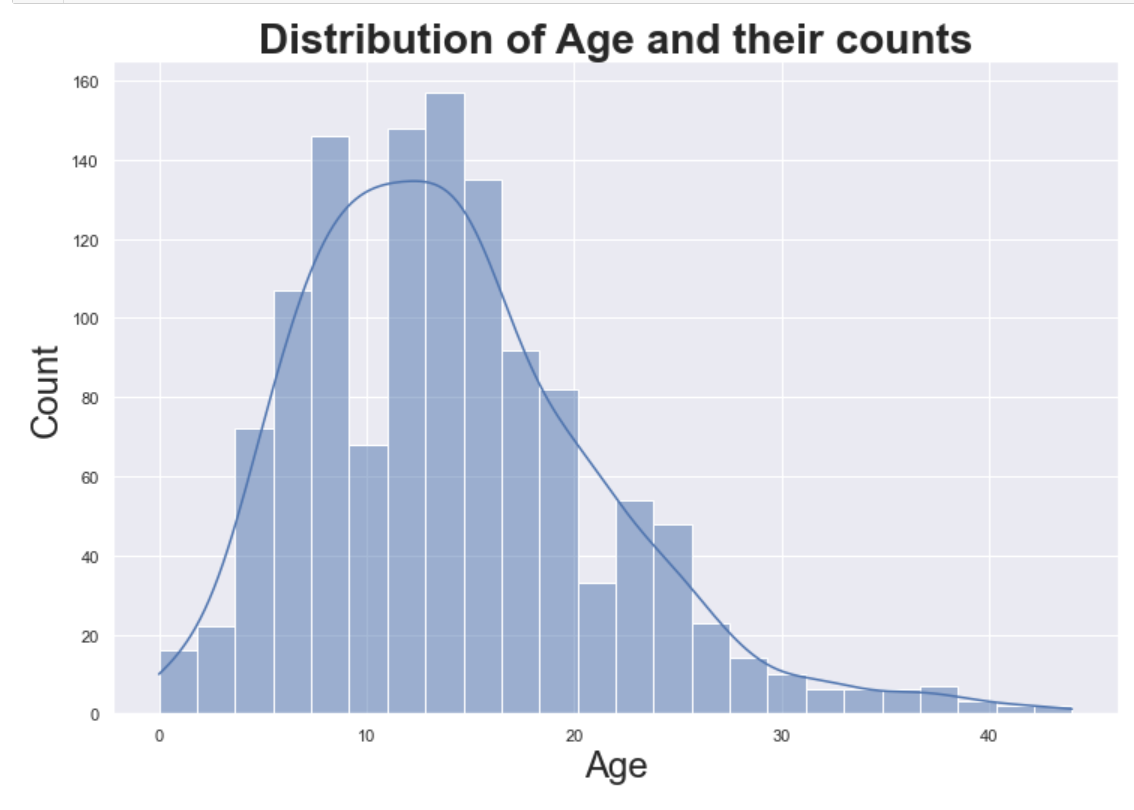
\includegraphics[width=3.5in]{1.png}
\caption{Histogram showing distribution of persons over age}
\end{figure}


\begin{figure}[h]
\centering
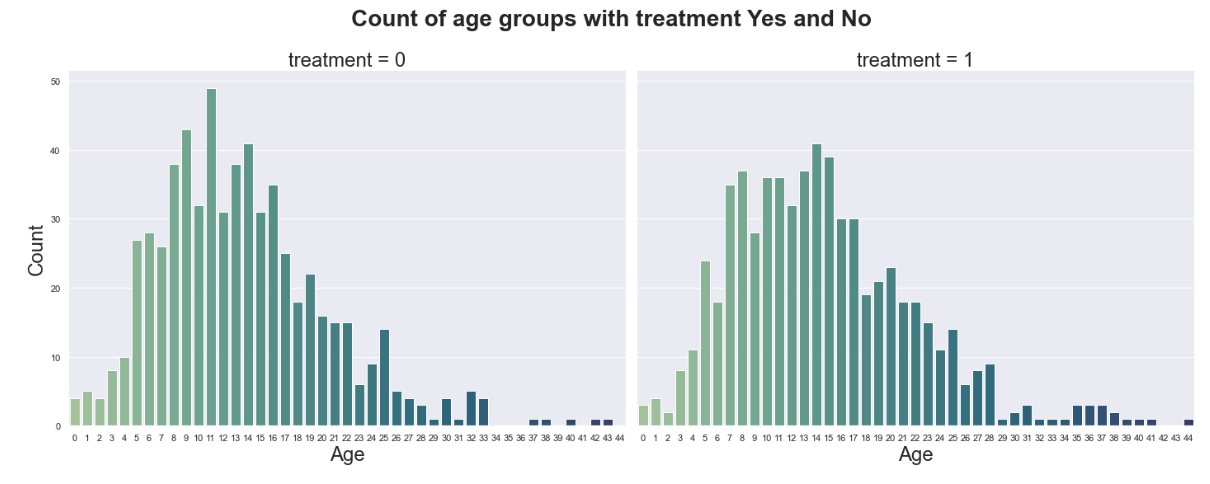
\includegraphics[width=3.5in]{2.png}
\caption{Plot showing the count of age groups who require treatment and not}
\end{figure}

\begin{figure}[h]
\centering
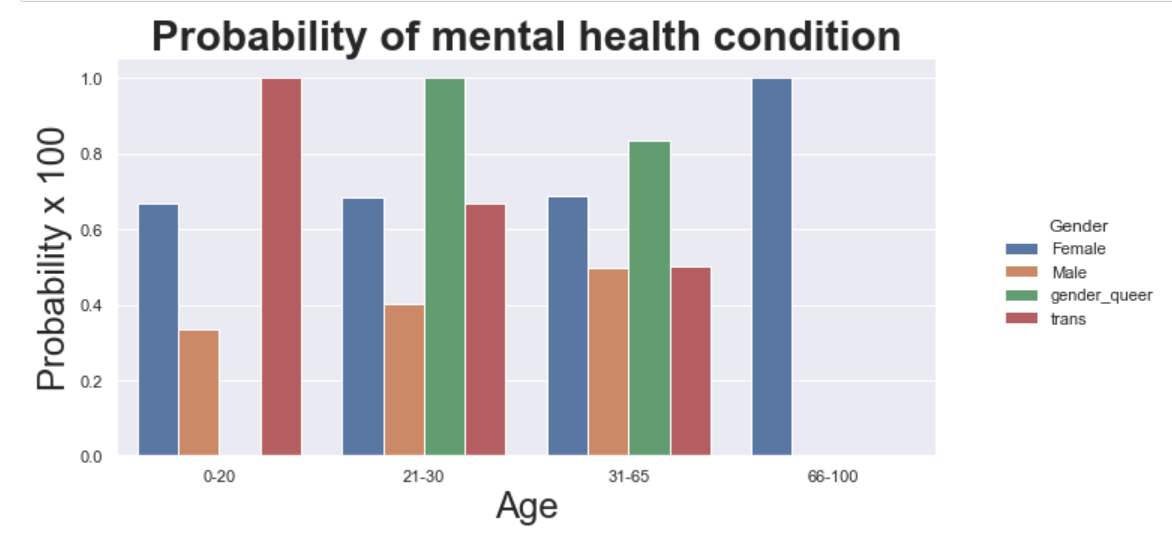
\includegraphics[width=3.5in]{3.png}
\caption{Probability of mental health conditions over age}
\end{figure}

\begin{figure}[h]
\centering
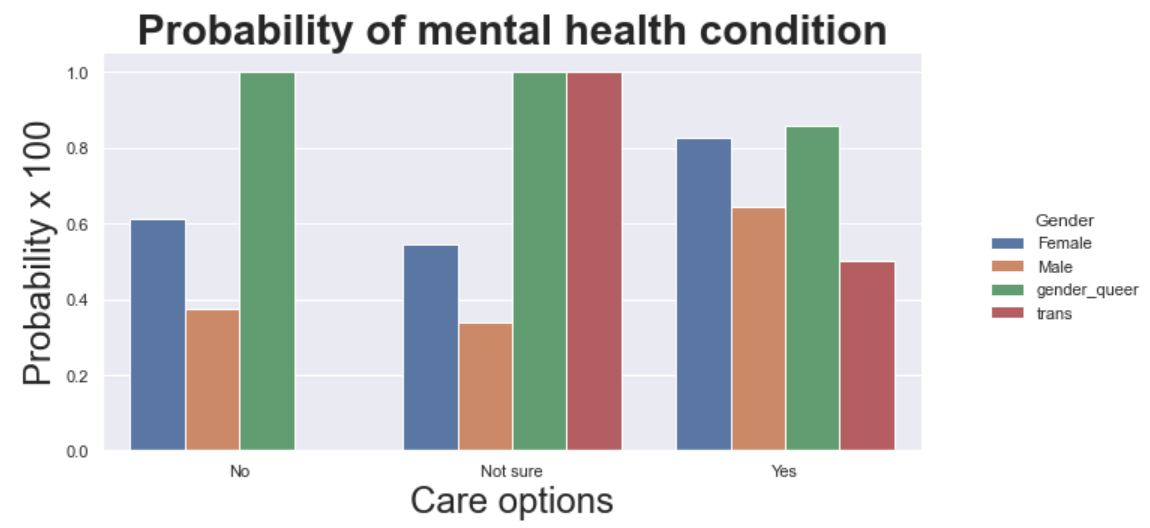
\includegraphics[width=3.5in]{4.png}
\caption{Probability of mental health conditions over care options}
\end{figure}


\quad  Nested barplots visualizing probability of mental health condition clearly show that in ages 0-20 Trans gender, gender queer in 21-30 and female in old ages have most probability.


\subsection{Data cleaning}
Dropping columns - Some of the features like Timestamp, state and comments do not contribute towards the classification. Furthermore, state and comments have large missing values. Hence it would be logical to drop these columns when classifying the data.

\quad Handling missing values: On dropping the two main missing value columns we were left with self\_employed and work\_interfere to handle the missing values. This is handled by assigning ‘No’ to the self\_employed column in missing places based on our exploration of records. For handling work\_interfere we added a new entry named Don’t Know for records with missing values.

\quad Handling outliers: The age column has 4 outliers which are handled by replacing the outliers with the column's median age.

\quad The gender column had different entries which had spelling mistakes, short forms, synonymous words, etc. We had to normalize all the entries into a few sub-groups like Male, Female, Gender queer and Trans. 

\subsection{Data Pre-Processing}
A number of the features considered are categorical hence they are required to be encoded into numericals. Label encoder is used to encode the Treatment feature which is the y in case of the classification and min max scalers and binarizers are used for encoding the features.

\section{Problem solution}
\subsection{Algorithm design}
A number of Machine learning algorithms could be used for this classification provided the number of features are limited to avoid the curse of dimensionality. This limitation results in the reduction of possible features which could contribute in a way or other to the classification. This could be handles using quantum computers which are expensive and complex to run. The approach we have considered is Quantum enhanced ML to give the power of Quantum computers yet run them in a simple way.

\subsubsection{Quantum Support Vector Machines}
As we saw in traditional the advantage of using traditional SVM is to classify data points in multiple dimensions by moving from euclidean space to Hilbert space. However, it has certain limitations on the number of dimensions it can handle using the kernel trick, and optimizing the kernel trick is very difficult with traditional SVM. Here is where QSVM helps with keeping the data points in the quantum state which can be achieved by a swapping circuit and building the kernel of SVM from these quantum states. After calculating the Kernel matrix on the quantum computer they can train the Quantum SVM the same way as a classical SVM. 
\begin{figure}[h]
\centering
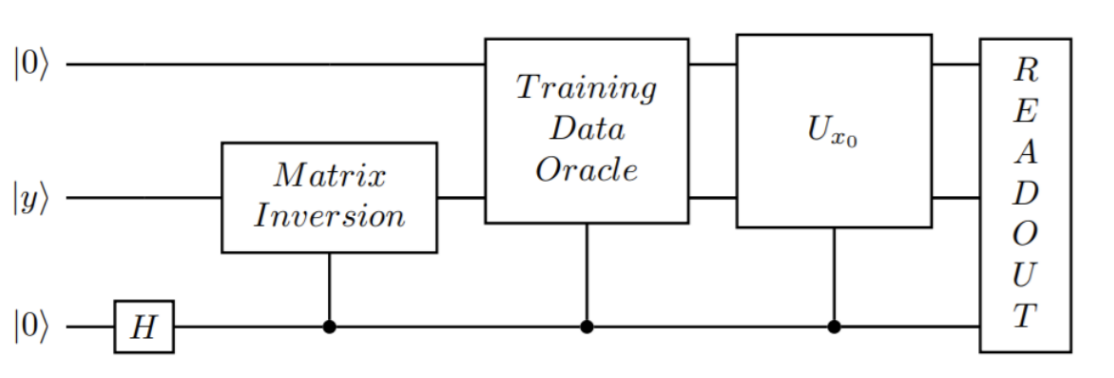
\includegraphics[width=3.5in]{6.png}
\caption{QSVM algorithm overview with readout}
\end{figure}

\quad The QSVM algorithm overview can be seen in Fig. 7 where three qubits where the first one is training register, second is input |y> state and third is ancilla qubit. 

\subsection{Modeling}
\subsubsection{Quantum SVM}
The Qiskit SDK package by IBMQ simulation products was used to implement the quantum variant of the traditional SVM. The documentation on the website is what was referred to while modeling the dataset. The QSVM approach is used for classification problems that call for a feature map but for which standard kernel computation is inefficient. As a result, it is anticipated that the needed computer resources will grow exponentially in proportion to the problem's size. In order to tackle this issue, QSVM directly estimates the kernel in the feature space using a quantum processor. The technique is characterized as "supervised learning," and it consists of a training phase (when the kernel is calculated and the support vectors are obtained) and a test or classification phase (where new data without labels is classified according to the solution found in the training phase). Depending on how many classes the data has, QSVM will internally perform a binary classification or a multiclass classification. If the data contains more than two classes, a multiclass extension must be provided. Below are the steps performed while implementing the algorithm. 1) Perform train, and test split on our dataset. 2) Plot the feature maps. 3) assign a feature map, and calculate the fidelity. 4) Select an SVM kernel. 5) fit and test the QSVM. 

\begin{figure}[h]
\centering
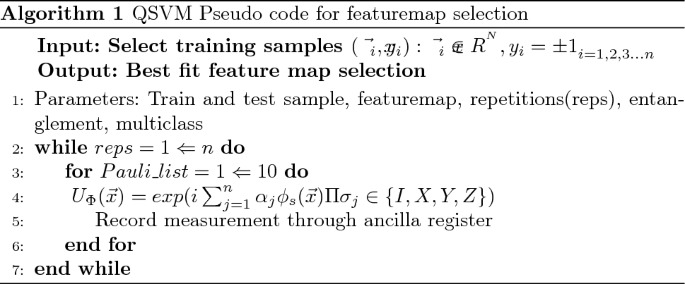
\includegraphics[width=3.5in]{code1.jpeg}
\caption{First algorithm in quantum variational support vector machine}
\end{figure}

\subsection{Evaluation metrics}
Our classification performance was planned to be measured using a number of metrics namely accuracy, precision, recall, and F1 score. However the qiskit library we used had not many metrics and we had to settle with the accuracy score alone. Lets look at the metrics which could be used for evaluation. The general terms for any prediction would be True Positive (TP), True Negatives (TN), False Positive (FP) and False Negative (FN)
Conditional Positive = P = TP + FN	
Conditional Negative = N = FP + TN

\subsubsection{Accuracy}
Accuracy can be seen as the closeness to the true values of the measured quantity. It mainly measures the statistical bias. It considers both the positive and negative samples being classified, thereby measuring the ability to classify positive samples in model.

Accuracy = (TN + TP) / (TN+TP+FN+FP) 
       = (TN + TP) / (P + N)		
       
\subsubsection{Precision}
Precision is measure of reproducibility of the measurement. It is a measure of statistical variability.

Precision = (TP)/(TP+FP)

\subsubsection{Recall}
Recall identifies accurately classifying all positive samples while ignoring if any negative samples classified as positive. It considers only the positive classifications while ignoring all negative samples. This allows us to identify how many positive classifications are made.

Recall = (TP)/(TP+FN)

\subsubsection{F1 score}
This is a combined measure of precision and recall of a classification model as a harmonic mean. This is the best way to compare two models when a decision cannot be made based on the recall and precision.

F1 = 2*(precision * recall)/(precision + recall)

\subsection{Model comparision}
QSVM has shown a pretty good performance with a score of 0.9 for the mental health dataset when 10 features where considered. On the other hand conventional SVM gave a  training accuracy of 0.72 but a very low testing accuracy of 0.50 for the same 10 features.

\subsection{Languages Used}
The project is developed in Python Programming Language. Core modeling of algorithms SVM is implemented in Python. 

\subsection{Tools used}
Google colab notebook is used for executing the models. Sklearn is used for preprocessing of data, matplotlib and Seaborn are used for visualizations, Qiskit is used for Quantum powering the models and sklearn models for comparision of performance.

% An example of a floating figure using the graphicx package.
% Note that \label must occur AFTER (or within) \caption.
% For figures, \caption should occur after the \includegraphics.
% Note that IEEEtran v1.7 and later has special internal code that
% is designed to preserve the operation of \label within \caption
% even when the captionsoff option is in effect. However, because
% of issues like this, it may be the safest practice to put all your
% \label just after \caption rather than within \caption{}.
%
% Reminder: the "draftcls" or "draftclsnofoot", not "draft", class
% option should be used if it is desired that the figures are to be
% displayed while in draft mode.
%
%\begin{figure}[!t]
%\centering
%\includegraphics[width=2.5in]{myfigure}
% where an .eps filename suffix will be assumed under latex, 
% and a .pdf suffix will be assumed for pdflatex; or what has been declared
% via \DeclareGraphicsExtensions.
%\caption{Simulation results for the network.}
%\label{fig_sim}
%\end{figure}

% Note that the IEEE typically puts floats only at the top, even when this
% results in a large percentage of a column being occupied by floats.
% However, the Computer Society has been known to put floats at the bottom.


% An example of a double column floating figure using two subfigures.
% (The subfig.sty package must be loaded for this to work.)
% The subfigure \label commands are set within each subfloat command,
% and the \label for the overall figure must come after \caption.
% \hfil is used as a separator to get equal spacing.
% Watch out that the combined width of all the subfigures on a 
% line do not exceed the text width or a line break will occur.
%
%\begin{figure*}[!t]
%\centering
%\subfloat[Case I]{\includegraphics[width=2.5in]{box}%
%\label{fig_first_case}}
%\hfil
%\subfloat[Case II]{\includegraphics[width=2.5in]{box}%
%\label{fig_second_case}}
%\caption{Simulation results for the network.}
%\label{fig_sim}
%\end{figure*}
%
% Note that often IEEE papers with subfigures do not employ subfigure
% captions (using the optional argument to \subfloat[]), but instead will
% reference/describe all of them (a), (b), etc., within the main caption.
% Be aware that for subfig.sty to generate the (a), (b), etc., subfigure
% labels, the optional argument to \subfloat must be present. If a
% subcaption is not desired, just leave its contents blank,
% e.g., \subfloat[].


% An example of a floating table. Note that, for IEEE style tables, the
% \caption command should come BEFORE the table and, given that table
% captions serve much like titles, are usually capitalized except for words
% such as a, an, and, as, at, but, by, for, in, nor, of, on, or, the, to
% and up, which are usually not capitalized unless they are the first or
% last word of the caption. Table text will default to \footnotesize as
% the IEEE normally uses this smaller font for tables.
% The \label must come after \caption as always.
%
%\begin{table}[!t]
%% increase table row spacing, adjust to taste
%\renewcommand{\arraystretch}{1.3}
% if using array.sty, it might be a good idea to tweak the value of
% \extrarowheight as needed to properly center the text within the cells
%\caption{An Example of a Table}
%\label{table_example}
%\centering
%% Some packages, such as MDW tools, offer better commands for making tables
%% than the plain LaTeX2e tabular which is used here.
%\begin{tabular}{|c||c|}
%\hline
%One & Two\\
%\hline
%Three & Four\\
%\hline
%\end{tabular}
%\end{table}


% Note that the IEEE does not put floats in the very first column
% - or typically anywhere on the first page for that matter. Also,
% in-text middle ("here") positioning is typically not used, but it
% is allowed and encouraged for Computer Society conferences (but
% not Computer Society journals). Most IEEE journals/conferences use
% top floats exclusively. 
% Note that, LaTeX2e, unlike IEEE journals/conferences, places
% footnotes above bottom floats. This can be corrected via the
% \fnbelowfloat command of the stfloats package.




\section{Conclusion}
The conclusions should only be regarded with a grain of salt because these results were computed on a small dataset with n = 10 dimensions and were somewhat random.
When quantum computing becomes more widely available, we might need to perform a cost analysis to determine whether the advantage is worthwhile or not. Physical quantum computers are now only available to academics and collaborators at accredited institutions, not to the general public.
As a result of the notion of an improved quantum feature space, machine learning can thus benefit from quantum computing.

\quad Recognizing that modern quantum computers are highly vulnerable to noise and physical perturbations during calculations is another crucial concern. Decoherence is a significant issue as well since it will not be practicable if physical quantum computing is ever made available to the majority of researchers. Today's quantum computers frequently lose or collapse quantum information.

% if have a single appendix:
%\appendix[Proof of the Zonklar Equations]
% or
%\appendix  % for no appendix heading
% do not use \section anymore after \appendix, only \section*
% is possibly needed

% use appendices with more than one appendix
% then use \section to start each appendix
% you must declare a \section before using any
% \subsection or using \label (\appendices by itself
% starts a section numbered zero.)
%

\appendices
\section{Criteria met in Rubrics}
1. Visualizations - During the exploratory data analysis phase a number of visualizations are used to understand the data and show correlations.

2. Presentation skills - We have practiced to maintain and cover important processes and concepts involved in our project by allotting enough time for questions.

3.Significance to the real world - This project is towards a social cause to bring awareness and in a way help people to understand their mental health condition The outcome of the project will inspire a similar idea of using QEML for other social causes and will improve the performance of traditional ML algorithms with the help of QEML. 

4. Saving the model for quick demo - Our models have been saved and can be loaded for testing and demo purpose. We have used picking approach where the trained model is saved as a file and later which can be loaded and test data can be run.

5. Code Walkthrough - The complete code is available in the colab notebook with clear comments making it easy to understand and elaborating the operations performed.

6. Report - We have strictly adhered to IEEE format for our report while taking care of the language and keeping it our own work. The report includes all the details required to understand our problem and approach towards solving it.

7. Version Control - Our entire data and code is maintained in Github repository with readme file.

8. Discussion / Q&A - Throughout the presentation, the discussion would be open and questions would be answered. There will be some time allocated for Q&A session in the end of the demo.

9. Lessons learned - The project is selected to be an added knowledge to our learning. With the understanding from the class curriculum about SVM we have extended thier applications in Quantum enhanced ML. Literature review, background, conclusions and comparisions all of the sections include the learnings from the project.

10. Prospects of winning competition / publication - QEML is a topic still under research and needs a lot of researchers to contribute. This could be a potential paper for publication as a very few references are available on QEML based models and especially for our classification problem. With some improvements in our approach this can be in future capable of a competition.

11. Innovation - QEML is a very new concept that needs to come into light. Our project is an implementation of this rarely explored concept to a social cause. We attempted to implement few algorithms that weren't previously available which could be seen as an area of future research.

12. Evaluation of Performance - The models are checked on an evaluation metric. Initially the correlations were checked which was a partial evaluation and later a comparision is made between models performance.

13. Teamwork - The whole team was involved in each phase of the project and had a weekly sync up to discuss progress towards the goal. A clear credit statement is mentioned in Appendix B.

14. Technical difficulty - As the topic is pretty new, less number of research papers were available to refer to and not many have addressed the problem or use case, also this requires the implementation of complex python libraries which simulate Quantum Computing power. A very few traditional machine-learning algorithms are implemented using this QEML method hence the modeling phase took a reasonably longer time. We have tried to implement few other models which weren't available in the library which was pretty difficult and had to drop them.

15. Practiced pair programming - GitHub copilot is used as a plugin in VScode.

16. Practiced agile / scrum (1-week sprints) - We followed a 1 week sprints agile framework using JIRA. Weekly meetings were held to track our progress on the deliverables.

17. Used Grammarly for language - We have used Grammarly to check our document language and rules.

18. Slides - Prepared our presentation slides to cover important aspects of the project.

19. Demo - We have prepared a demo structure to follow for a better presentation and show the working model.

20. Using LaTEX - We have used laTex for formatting our report using the IEEE template. All the documentation is done using overleaf.

21. Used creative presentation techniques - The presentation slides are prepared with the Prezi tool with interesting animations.

22. Literature Survey - We have referred to papers and research that cover mental health predictions and classifications. All the literature is distributed into meaningful subsections and concepts are introduced appropriately. Al the cited works are referred.

\section{Author Contributions}
Sadakhya Narnur: Conceptualization, Methodology, Investigation, Writing – Original Draft.
Neha Shaikh: Software, Validation, Data Curation, Writing – Review and Editing.
Rahul Reddy Parupati: Visualization, Formal analysis, Validation, Writing – Review and Editing.
Praveen Kumar Thanniru : Project administration, Investigation, Writing – Review and Editing.

% use section* for acknowledgment
\ifCLASSOPTIONcompsoc
  % The Computer Society usually uses the plural form
  \section*{Acknowledgments}
\else
  % regular IEEE prefers the singular form
  \section*{Acknowledgment}
\fi


The authors would like to thank Professor Dr. Vishnu Pendyala, Nikita Balani and Vineeth Reddy Chintala for being supportive throughout the process. This work is done as a part of Machine Learning Technologies course work.

% Can use something like this to put references on a page
% by themselves when using endfloat and the captionsoff option.
\ifCLASSOPTIONcaptionsoff
  \newpage
\fi



% trigger a \newpage just before the given reference
% number - used to balance the columns on the last page
% adjust value as needed - may need to be readjusted if
% the document is modified later
%\IEEEtriggeratref{8}
% The "triggered" command can be changed if desired:
%\IEEEtriggercmd{\enlargethispage{-5in}}

% references section

% can use a bibliography generated by BibTeX as a .bbl file
% BibTeX documentation can be easily obtained at:
% http://mirror.ctan.org/biblio/bibtex/contrib/doc/
% The IEEEtran BibTeX style support page is at:
% http://www.michaelshell.org/tex/ieeetran/bibtex/
%\bibliographystyle{IEEEtran}
% argument is your BibTeX string definitions and bibliography database(s)
%\bibliography{IEEEabrv,../bib/paper}
%
% <OR> manually copy in the resultant .bbl file
% set second argument of \begin to the number of references
% (used to reserve space for the reference number labels box)
\begin{thebibliography}{1}

\bibitem{1}
Sumathi, M. R., and B. Poorna. "Prediction of mental health problems among children using machine learning techniques." International Journal of Advanced Computer Science and Applications 7.1 (2016).

\bibitem{2}
Vaishnavi, Konda, et al. "Predicting Mental Health Illness using Machine Learning Algorithms." Journal of Physics: Conference Series. Vol. 2161. No. 1. IOP Publishing, 2022.

\bibitem{3}
Thomas, Dr G., Krishna Sai Mangalarapu, Munawar Ali Md, and Vamsi Krishna Talakokkula. "A New Quantum Approach to Binary Classification." arXiv preprint arXiv:2106.15572 (2021).

\bibitem{4}
Kariya, Anekait, and Bikash K. Behera. "Investigation of Quantum Support Vector Machine for Classification in NISQ era." arXiv preprint arXiv:2112.06912 (2021).

\bibitem{5}
Chirag Dodiya.2021. Mental-Health-Prediction-using-Machine-Learning-Algorithms. https://github.com/cdodiya/Mental-Health-Prediction-using-Machine-Learning-Algorithms/blob/main/survey.csv(2022)

\end{thebibliography}

% biography section
% 
% If you have an EPS/PDF photo (graphicx package needed) extra braces are
% needed around the contents of the optional argument to biography to prevent
% the LaTeX parser from getting confused when it sees the complicated
% \includegraphics command within an optional argument. (You could create
% your own custom macro containing the \includegraphics command to make things
% simpler here.)
%\begin{IEEEbiography}[{\includegraphics[width=1in,height=1.25in,clip,keepaspectratio]{mshell}}]{Michael Shell}
% or if you just want to reserve a space for a photo:

% if you will not have a photo at all:
\begin{IEEEbiographynophoto}{Neha Shaikh}
is currently pursuing a Master of Science in Data Analytics. The main research areas include sentiment analysis, enhancing ML algorithms, and drug discovery.
Passionate about using ML for social good. 
\end{IEEEbiographynophoto}


\begin{IEEEbiographynophoto}{Praveen Kumar}
is currently pursuing a Master of Science in Data Analytics.
\end{IEEEbiographynophoto}

\begin{IEEEbiographynophoto}{Sadakhya Narnur}
is currently pursuing a Master of Science in Data Analytics. Her main research interests include Object Detection and prediction \& analytics in the field of medicine.
\end{IEEEbiographynophoto}

\begin{IEEEbiographynophoto}{Rahul Reddy Parupati}
is currently pursuing a Master of Science in Data Analytics.
\end{IEEEbiographynophoto}

% You can push biographies down or up by placing
% a \vfill before or after them. The appropriate
% use of \vfill depends on what kind of text is
% on the last page and whether or not the columns
% are being equalized.

%\vfill

% Can be used to pull up biographies so that the bottom of the last one
% is flush with the other column.
%\enlargethispage{-5in}



% that's all folks
\end{document}


